\documentclass[11pt,letterpaper]{article}


%% Language and font encodings
\usepackage{multicol}
\usepackage[english,spanish]{babel}
\usepackage[utf8x]{inputenc}
\usepackage[T1]{fontenc}
\usepackage{lmodern}

%% Sets page size and margins
\usepackage[top=3cm,bottom=2cm,left=3cm,right=3cm,marginparwidth=1.75cm]{geometry}

%% Useful packages
\usepackage{amsmath}
\usepackage{graphicx}
\usepackage[colorinlistoftodos]{todonotes}
\usepackage[colorlinks=true, allcolors=black]{hyperref}
\usepackage{titlesec}
\titlespacing*{\section}{0pt}{1.0ex}{3.0ex}
\usepackage{enumitem}   % listas compactas
\setlist{itemsep=2pt, topsep=4pt, leftmargin=*}

\setlength{\parskip}{0pt}
\setlength{\parindent}{15pt}

\usepackage{booktabs}
\usepackage{caption}
\captionsetup{font=small,labelfont=bf}
\setlength{\parskip}{0pt}
\setlength{\parindent}{15pt}
\addto\captionsspanish{\renewcommand{\tablename}{Tabla}}

% Marca en rojo lo que falta completar (bórrala al terminar)
\newcommand{\pendiente}[1]{\textcolor{red}{[#1]}}

\usepackage{float}

\setlength{\intextsep}{6pt plus 2pt minus 2pt}
\setlength{\floatsep}{6pt plus 2pt minus 2pt}
\setlength{\textfloatsep}{8pt plus 2pt minus 4pt}
\setlength{\abovecaptionskip}{4pt}
\setlength{\belowcaptionskip}{0pt}

\begin{document}

\thispagestyle{empty}
\begin{center}
\begin{figure}[h]
\centering

\includegraphics[width=.6\textwidth]{logo.jpg}\\
\end{figure}

\vspace{3.5cm}
\Large \sc  Eliminación de artefactos en imágenes de endoscopía
\\

\vspace{3.2cm}

\emph{Avance 2. Resultados de la prueba 1}

\vspace{3.2cm}

\Large {Equipo}\\
\vspace{0.3cm}
\Large \bf Mario Raúl García Ramírez - A01658682\\
\vspace{0.3cm}
\Large Javier Emmanuel García Escobedo - A01411206\\
\vspace{0.3cm}
\Large Juan Miguel Molina Reyes - A01796655\\
\vspace{1.2cm}
\normalfont\normalsize \textbf{Profesor:} Dr.Gilberto Ochoa Ruiz, EIC Computación \\
\vspace{0.2cm}
\normalsize \textbf{Patrocinador:} Dr. Gerardo Jesús Camacho González, INSiDE Lab\\
\vspace{1.5cm}
\normalsize \sc \rightline{Proyecto Integrador}
\vspace{0.0cm}
\normalsize \sc \rightline{11 de Octubre del 2026}
\end{center}

\newpage

\tableofcontents
\clearpage

\raggedcolumns
\begin{multicols}{2}

% =====================================================
\section{Prueba 1: Pipeline completo sobre C3VDv2}
% =====================================================

\subsection{Objetivo e hipótesis}
La Prueba 1 es la primera corrida completa del pipeline del proyecto con datos reales: Endo-STTN \cite{Daher2023} limpia los reflejos especulares de los frames, un estimador de profundidad se ajusta con la profundidad real del conjunto de datos y se evalúa contra esa misma referencia. Su propósito es doble: (1) comprobar que el pipeline funciona de extremo a extremo con una muestra pequeña del conjunto C3VDv2 \cite{Golhar2025,C3VDData}, y (2) obtener una primera estimación del efecto de limpiar los reflejos sobre la estimación de profundidad.

La hipótesis es que un estimador de profundidad entrenado y evaluado con frames limpiados comete menos error que uno entrenado y evaluado con frames originales, sobre todo dentro y alrededor de los reflejos.

\subsection{Configuración experimental}
\paragraph{Datos y partición.} La Tabla~\ref{tab:config} resume la configuración. Se usaron cinco videos de C3VDv2 (tres de entrenamiento, uno de validación y uno de prueba). Cada video se submuestreó a 1 de cada 5 frames (hasta 300 por video) y se redimensionó a $320\times256$. La profundidad real, almacenada como TIFF de 16 bits, se convirtió a milímetros (0--100~mm; los valores 0 y 65535 se tratan como ``sin dato''). La máscara de reflejos marca los píxeles con brillo (escala de grises) mayor o igual a 230, dilatados 3~px a $320\times256$. La partición se hace por video (nunca por frame): el código fija listas de videos de prueba y de validación y asigna a entrenamiento todos los demás videos disponibles.

\begin{table}[H]
\centering
\scriptsize
\caption{Configuración de la Prueba 1.}
\label{tab:config}
\begin{tabular}{@{}p{1.9cm}p{5.3cm}@{}}
\toprule
Fecha / entorno & 11 oct. 2026; Google Colab, GPU Tesla T4 \\
Entrenamiento & \texttt{c2\_\allowbreak descending\_\allowbreak t4\_\allowbreak v1}, \texttt{c2\_\allowbreak descending\_\allowbreak t4\_\allowbreak v2}, \texttt{c2\_\allowbreak rectum\_\allowbreak t1\_\allowbreak v1} \\
Validación & \texttt{c2\_\allowbreak descending\_\allowbreak t3\_\allowbreak v1} (elige la mejor época) \\
Prueba & \texttt{c2\_\allowbreak descending\_\allowbreak t4\_\allowbreak v3} (26 frames) \\
Limpieza & Endo-STTN preentrenado (\texttt{gen\_\allowbreak 00009.pth}), sin entrenar; solo modifica píxeles de reflejo \\
Estimador & AF-SfMLearner \cite{Shao2022}, pesos \textit{End-to-end} preentrenados en SCARED \cite{Allan2021} \\
Ajuste fino & Pérdida \textit{scale-invariant log}; Adam, lr $10^{-4}$ (decoder) y $10^{-5}$ (encoder); lote 8; 15 épocas; semilla 0 \\
\bottomrule
\end{tabular}
\end{table}

\paragraph{Variantes comparadas.} Se evalúan cuatro modelos que combinan el estimador (con pesos de SCARED o ajustado en C3VDv2) con el tipo de frame de entrada (originales o limpiados):

\begin{table}[H]
\centering
\scriptsize
\caption{Variantes de modelo evaluadas.}
\label{tab:variantes}
\begin{tabular}{@{}clll@{}}
\toprule
 & Pesos & Entrada & Ajuste fino con \\
\midrule
A & SCARED & originales & --- \\
B & SCARED & limpios & --- \\
C & ajustado & originales & originales \\
D & ajustado & limpios & limpios \\
\bottomrule
\end{tabular}
\end{table}



\subsection{Pasos del Pipeline}
\begin{enumerate}
\item \textbf{Preparación de datos.} Submuestreo, redimensionado, conversión de profundidad y cálculo de máscaras (Figura~\ref{fig:frame}).
\item \textbf{Limpieza.} Endo-STTN sustituye los píxeles de reflejo. La verificación del notebook confirma que \textbf{0 píxeles cambiaron fuera de la máscara}, es decir, la limpieza no altera el resto de la imagen (Figura~\ref{fig:limpieza}).
\item \textbf{Ajuste fino.} Se entrenan C (frames originales) y D (frames limpios) con la profundidad real; se conserva la época con menor AbsRel de validación.
\item \textbf{Evaluación.} Se evalúan A, B, C y D sobre los 26 frames de prueba con escalamiento por mediana (\textit{median scaling}) usando toda la imagen. Las métricas son AbsRel, SqRel, RMSE (mm), RMSE log y $\delta<1.25$, calculadas en tres regiones: toda la imagen, dentro de los reflejos y un anillo de 10~px alrededor de ellos. Las diferencias entre modelos se contrastan con la prueba de Wilcoxon pareada por frame.
\end{enumerate}

\begin{figure}[H]
\centering
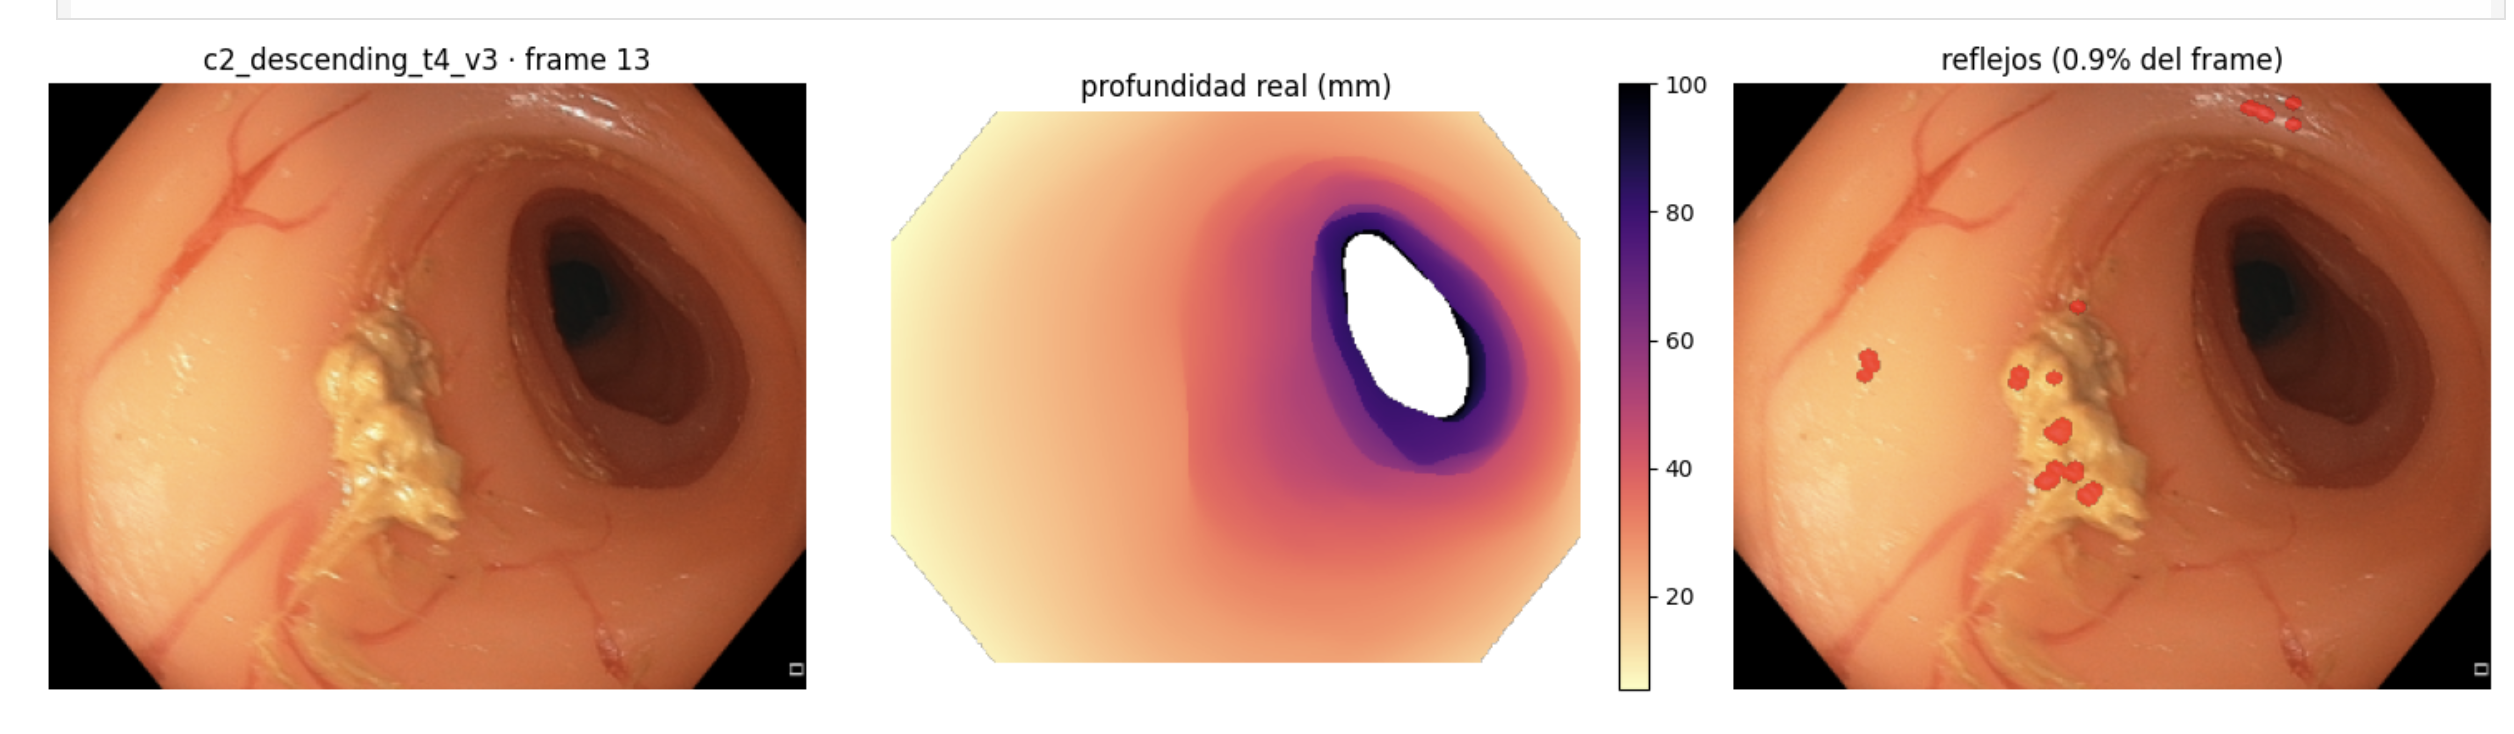
\includegraphics[width=\columnwidth]{frame_prueba.png}
\caption{Frame 13 del video de prueba: imagen, profundidad real (mm; en blanco, sin dato) y máscara de reflejos (0.9~\% del frame).}
\label{fig:frame}
\end{figure}

\begin{figure}[H]
\centering
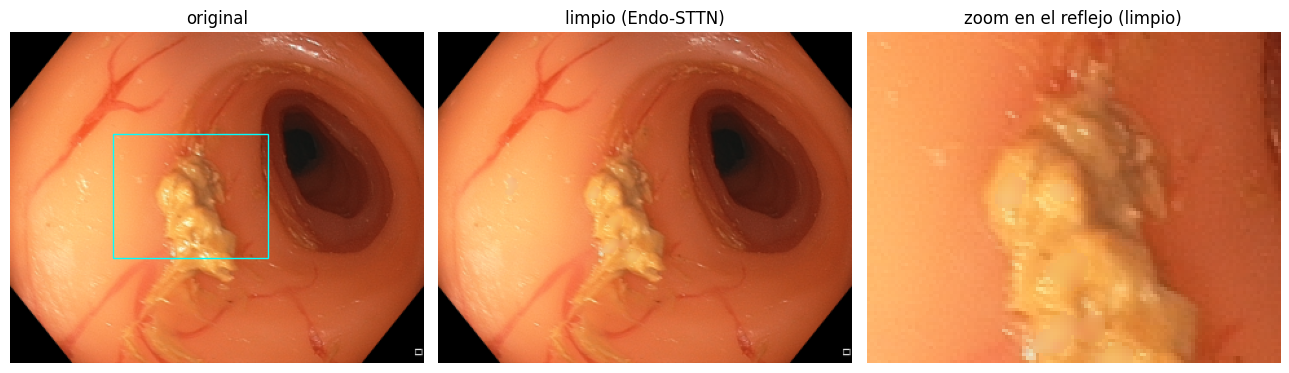
\includegraphics[width=\columnwidth]{limpieza.png}
\caption{Frame original, frame limpiado por Endo-STTN y detalle ampliado.}
\label{fig:limpieza}
\end{figure}

% =====================================================
\section{Resultados}
% =====================================================

\subsection{Error de profundidad por región}

La Tabla~\ref{tab:absrel} y la Figura~\ref{fig:absrel} muestran el AbsRel en el video de prueba.

\begin{table}[H]
\centering
\scriptsize
\caption{AbsRel en el video de prueba (menor es mejor).}
\label{tab:absrel}
\begin{tabular}{@{}lccc@{}}
\toprule
Modelo & Imagen & Reflejos & Anillo \\
\midrule
A (SCARED, orig.) & 0.404 & 0.753 & 0.476 \\
B (SCARED, limpios) & 0.399 & 0.744 & 0.457 \\
C (ajustado, orig.) & 0.089 & 0.111 & 0.104 \\
D (ajustado, limpios) & \textbf{0.078} & \textbf{0.085} & \textbf{0.075} \\
\midrule
Cambio C $\to$ D & $-12.4\,\%$ & $-23.0\,\%$ & $-27.8\,\%$ \\
\bottomrule
\end{tabular}
\end{table}

\begin{figure}[H]
\centering
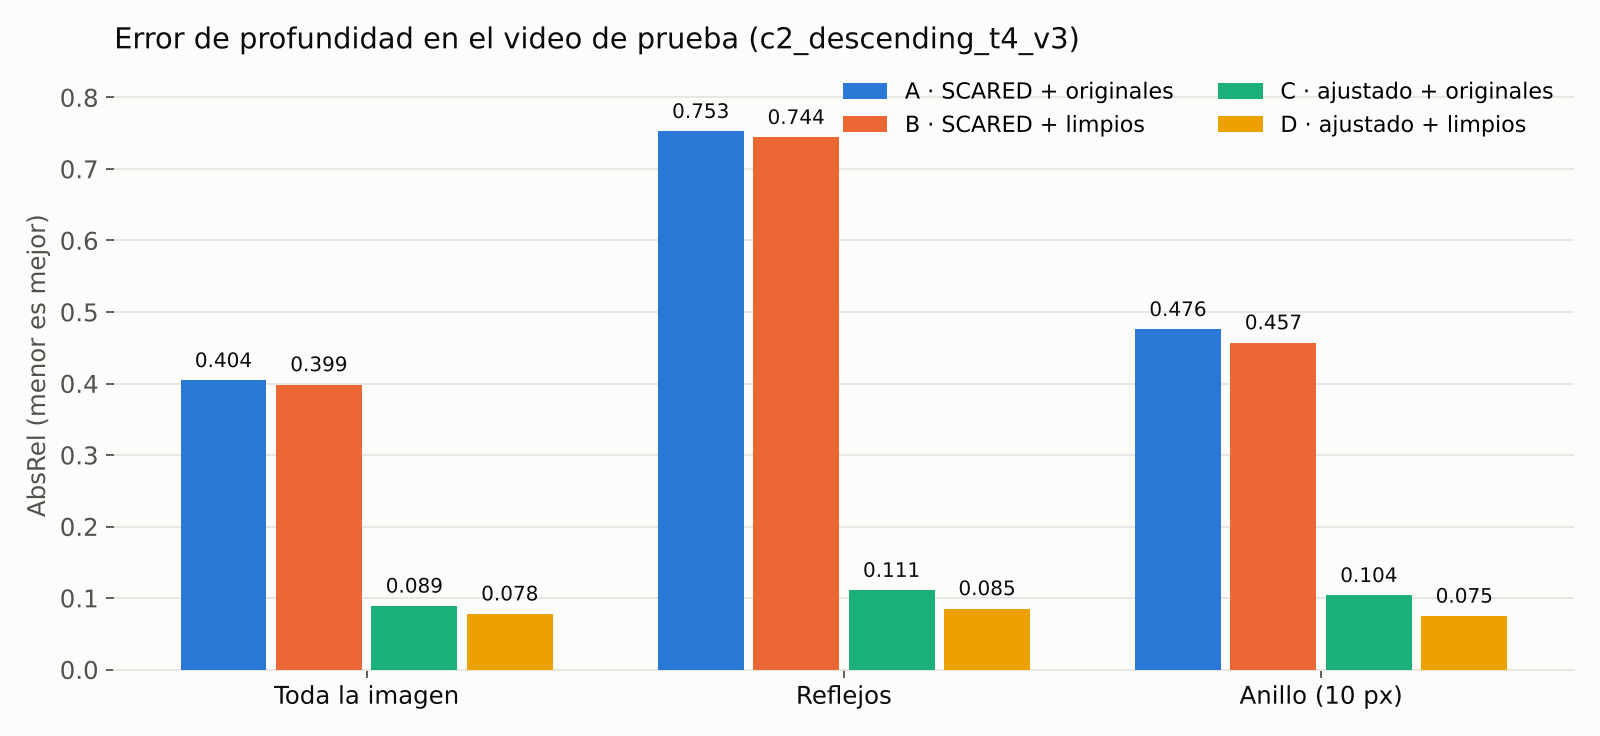
\includegraphics[width=.95\columnwidth]{absrel_por_region.png}
\caption{AbsRel por región y modelo.}
\label{fig:absrel}
\end{figure}

El ajuste fino reduce el AbsRel en toda la imagen de 0.404 (A) a 0.089 (C), una caída de 78~\%. Limpiar los frames sin reentrenar (A $\to$ B) mejora entre 1 y 4~\% según la región. Entrenar y evaluar con frames limpios (C $\to$ D) mejora más en las regiones de interés (reflejos y anillo) que en la imagen completa. La Figura~\ref{fig:pred} muestra las predicciones y los mapas de error de los cuatro modelos en un frame de prueba.

\begin{figure}[H]
\centering
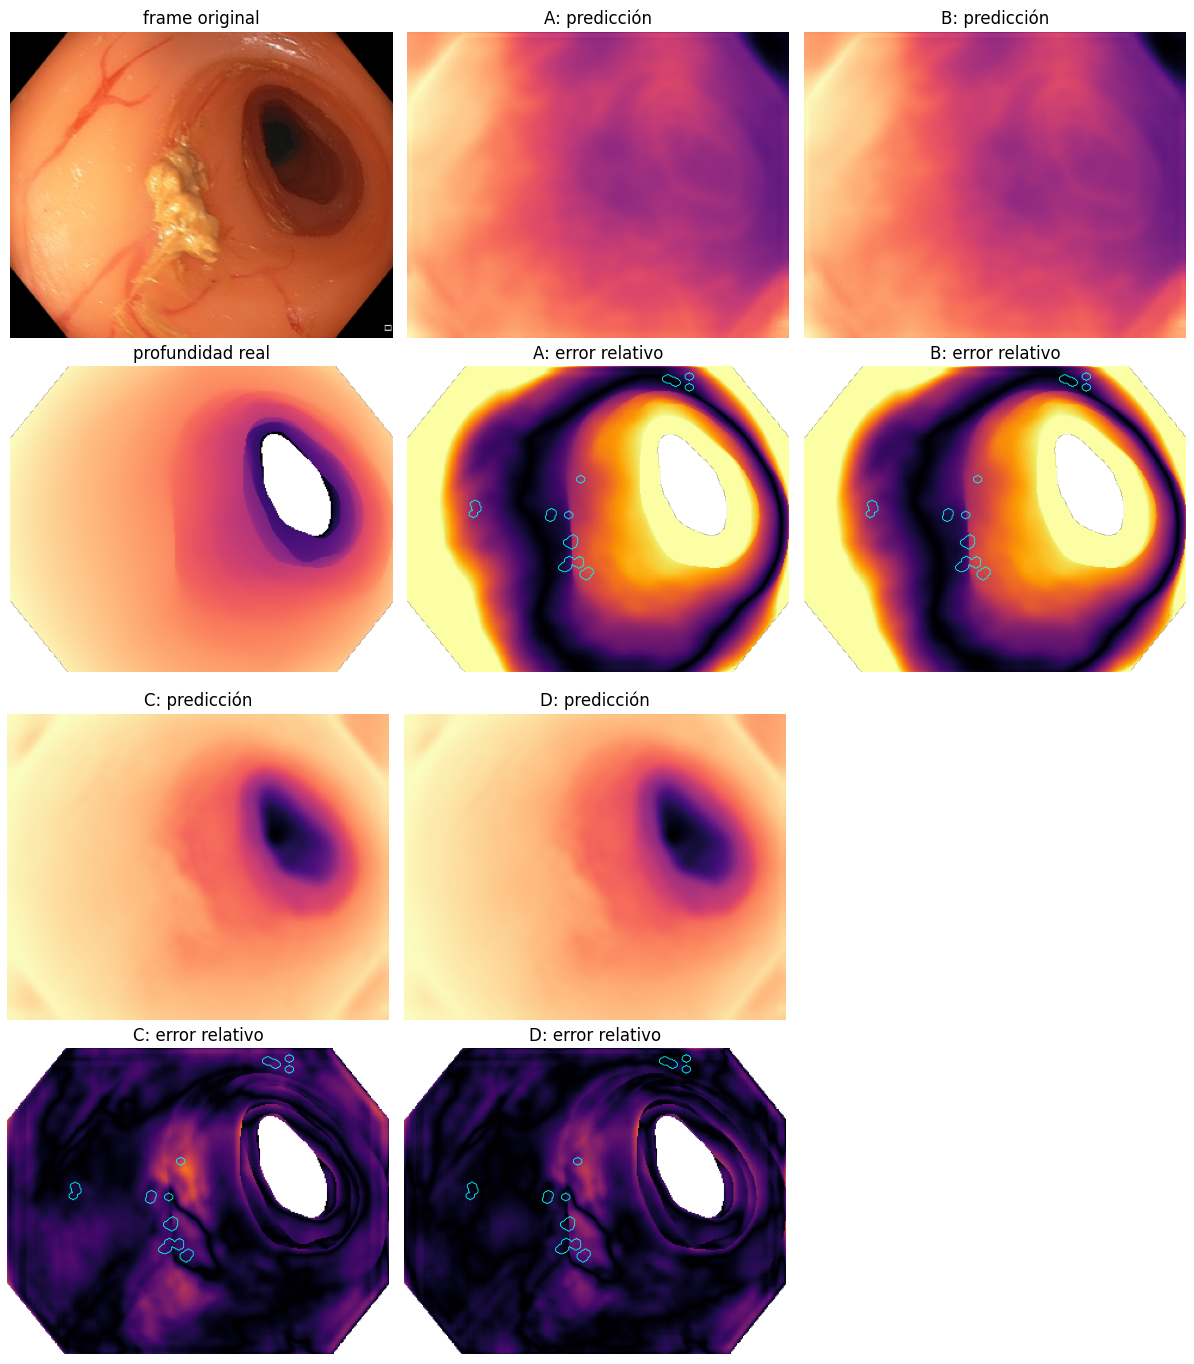
\includegraphics[width=\columnwidth]{predicciones_ABCD_2.png}
\caption{Profundidad predicha (arriba de cada bloque) y error relativo (abajo) de A--D en un frame de prueba; contornos: reflejos.}
\label{fig:pred}
\end{figure}

\subsection{Significancia por frame}

Se aplicó la prueba de Wilcoxon pareada sobre el AbsRel de los 26 frames (hipótesis alterna: el segundo modelo tiene menor AbsRel).

\begin{table}[H]
\centering
\scriptsize
\caption{Pruebas de Wilcoxon pareadas ($n=26$ frames).}
\label{tab:wilcoxon}
\begin{tabular}{@{}llcc@{}}
\toprule
Comparación & Región & Mediana dif. & $p$ \\
\midrule
C vs D & reflejos & 0.028 & 0.015 \\
C vs D & imagen & 0.018 & 0.0005 \\
A vs B & reflejos & 0.002 & 0.134 \\
\bottomrule
\end{tabular}
\end{table}

Las dos diferencias C vs D resultan significativas al nivel 0.05 y siguen por debajo del umbral de Bonferroni para tres pruebas ($0.05/3\approx0.017$), aunque la de reflejos lo hace por poco. La diferencia A vs B no es significativa. Estos valores de $p$ deben leerse con cautela (véase la Sección~\ref{sec:limit}).

\subsection{Otras métricas}

\begin{table}[H]
\centering
\scriptsize
\setlength{\tabcolsep}{3pt}
\caption{Métricas por región para los modelos ajustados (en negritas, el mejor).}
\label{tab:otras}
\begin{tabular}{@{}llccccc@{}}
\toprule
Región & Mod. & AbsRel & SqRel & RMSE & RMSE log & $\delta_1$ \\
\midrule
Imagen & C & 0.089 & 0.334 & \textbf{3.67} & 0.112 & 0.950 \\
 & D & \textbf{0.078} & \textbf{0.321} & 3.82 & \textbf{0.102} & \textbf{0.958} \\
Reflejos & C & 0.111 & 0.242 & 1.95 & 0.130 & \textbf{0.929} \\
 & D & \textbf{0.085} & \textbf{0.202} & \textbf{1.71} & \textbf{0.110} & 0.910 \\
Anillo & C & 0.104 & 0.243 & 2.04 & 0.125 & 0.925 \\
 & D & \textbf{0.075} & \textbf{0.176} & \textbf{1.72} & \textbf{0.101} & \textbf{0.931} \\
\bottomrule
\end{tabular}
\end{table}

\noindent RMSE en mm; $\delta_1$ denota $\delta<1.25$. Las tablas completas de A--D están en el archivo \texttt{evaluacion\_\allowbreak resumen.md} del repositorio.

\subsection{Curvas de validación}

En validación, C y D terminan prácticamente iguales (mejor AbsRel de 0.156 y 0.154, respectivamente); D desciende más rápido entre las épocas 3 y 7 (Figura~\ref{fig:curvas}). El AbsRel de validación (cercano a 0.155) es casi el doble del obtenido en prueba (0.078--0.089), diferencia que se discute en la Sección~\ref{sec:fuga}.

\begin{figure}[H]
\centering
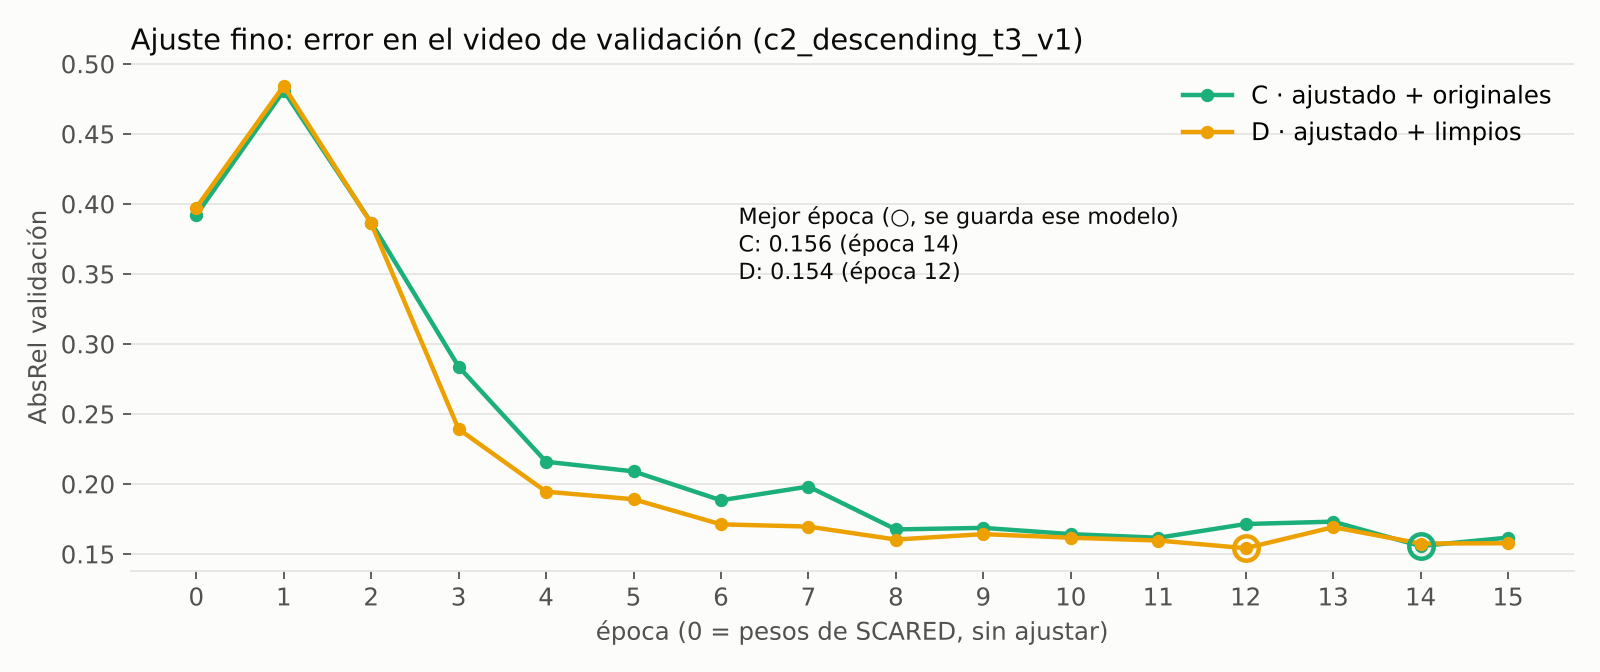
\includegraphics[width=\columnwidth]{curvas_validacion.png}
\caption{AbsRel de validación por época para C y D.}
\label{fig:curvas}
\end{figure}

% =====================================================
\section{Interpretación}
% =====================================================

\begin{enumerate}
\item \textbf{El ajuste fino pesa más que la limpieza.} AF-SfMLearner, entrenado en SCARED (tejido porcino), no se transfiere bien a los modelos de silicona de C3VDv2 sin adaptación (A $\to$ C: $-78\,\%$ de AbsRel).
\item \textbf{Limpiar ayuda cuando el estimador aprende con frames limpios.} D mejora a C en casi todas las métricas, y más en reflejos y anillo, lo cual es coherente con la hipótesis.
\item \textbf{Limpiar sin reentrenar aporta poco.} B frente a A mejora solo 1--4~\% y no es significativo ($p=0.134$); el beneficio parece requerir que el estimador se entrene con el mismo tipo de imagen que recibe.
\item \textbf{No todas las métricas favorecen a D.} El RMSE en toda la imagen (3.82 frente a 3.67~mm) y $\delta<1.25$ en reflejos (0.910 frente a 0.929) son ligeramente peores. D reduce el error relativo, pero no gana en todos los criterios.
\end{enumerate}

% =====================================================
\section{Limitaciones y validez de los resultados}
\label{sec:limit}
% =====================================================

\subsection{Fuga de información entre entrenamiento y prueba}
\label{sec:fuga}

La estrategia de muestreo del equipo establece que la partición debe hacerse por segmento del fantoma para evitar fuga de información (Estrategia de muestreo, \S1.4). En la Prueba 1 esa regla no se cumplió. La causa está en el código: \texttt{codigo/c3vd.py} reparte por video, con listas fijas de videos de prueba y de validación, y manda a entrenamiento todos los demás; no agrupa por segmento. Así, el video de prueba \texttt{c2\_\allowbreak descending\_\allowbreak t4\_\allowbreak v3} quedó junto con \texttt{t4\_\allowbreak v1} y \texttt{t4\_\allowbreak v2}, del mismo segmento (\texttt{c2\_\allowbreak descending\_\allowbreak t4}), en entrenamiento. Lo mismo ocurriría con cualquiera de los otros videos de prueba predefinidos si se descargan sus v1 o v2.

Los videos de un mismo segmento comparten fantoma y trayectoria. No se verificó cuánto se parecen sus mapas de profundidad, pero es esperable que sean muy similares. Dos indicios apuntan a que los valores absolutos son optimistas: el AbsRel de validación, en un video de otro segmento (\texttt{c2\_\allowbreak descending\_\allowbreak t3\_\allowbreak v1}), es cercano a 0.155, casi el doble del de prueba; y el propio README reconoce que prueba y entrenamiento comparten textura. Por eso, \textbf{las cifras absolutas (p.~ej., AbsRel 0.089) no deben interpretarse como el desempeño esperado en un segmento nuevo}, ni la magnitud de la mejora A $\to$ C como una medida de generalización. La comparación C vs D sigue siendo controlada, porque la misma partición afecta a ambos modelos por igual; sin embargo, no se puede descartar que parte de la ventaja de D dependa de esa cercanía entre entrenamiento y prueba.

\subsection{Otras limitaciones}

\paragraph{Tamaño de muestra y pruebas estadísticas.} Hay un solo video de prueba con 26 frames, y frames consecutivos están correlacionados, por lo que los valores de $p$ (que suponen observaciones independientes) son optimistas. Además, se hicieron tres pruebas sin corrección formal más allá de la comparación con el umbral de Bonferroni indicada arriba.

\paragraph{Una sola semilla.} No se conoce todavía cuánto varía la diferencia C--D con otra inicialización del entrenamiento.

\paragraph{Pocos datos de entrenamiento.} Solo se usaron tres videos de entrenamiento, de una misma región del colon y del recto.

\paragraph{Máscaras y métricas.} Las máscaras se obtienen por umbral de brillo (230) con dilatación de 3~px, por lo que pueden incluir también otros objetos brillantes distintos de los reflejos (p.~ej., residuos o moco), y se evalúan solo sobre los píxeles con profundidad válida. Además, la mejora no es uniforme en todas las métricas (Sección~3).

\paragraph{Entorno.} La prueba se ejecutó en Colab (Tesla T4), con un entorno distinto al de los autores de Endo-STTN; los valores de referencia del artículo original no son directamente comparables con los de esta prueba.

% =====================================================
\section{Siguientes pasos}
% =====================================================

Los siguientes puntos son propuestas para la Prueba 2 y quedan por acordar con el equipo:

\begin{enumerate}
\item \textbf{Criterio de partición.} Revisar el criterio de partición frente a la Estrategia de muestreo (\S1.4), de modo que los videos de prueba no compartan segmento con los de entrenamiento. En particular, \texttt{c2\_\allowbreak rectum\_\allowbreak t1\_\allowbreak v3}, citado en el README como textura no vista, comparte segmento con \texttt{c2\_\allowbreak rectum\_\allowbreak t1\_\allowbreak v1}, usado para entrenar.
\item \textbf{Más semillas.} Repetir C y D con las semillas 1 y 2 y reportar media $\pm$ desviación estándar.
\item \textbf{Más videos de prueba y de entrenamiento}, incluyendo otras secciones del colon (p.~ej., \texttt{c1\_\allowbreak ascending\_\allowbreak *}).
\item \textbf{Análisis estadístico.} Aplicar una corrección por comparaciones múltiples y, de ser posible, agregar los resultados por video en lugar de por frame.
\end{enumerate}

% =====================================================
\section{Archivos y reproducibilidad}
% =====================================================

\begin{itemize}
\item \texttt{Equipo19\_\allowbreak Avance2\_\allowbreak colab\_\allowbreak ejecutado.ipynb}: notebook de Colab con todas las celdas ejecutadas.
\item \texttt{evaluacion\_\allowbreak resumen.md}: tablas completas A--D y pruebas de Wilcoxon (hay una versión \texttt{.csv} con las medias).
\item \texttt{evaluacion\_\allowbreak por\_\allowbreak frame.csv}: métricas de cada uno de los 26 frames.
\item \texttt{historial\_\allowbreak C\_\allowbreak rgb.json} y \texttt{historial\_\allowbreak D\_\allowbreak rgb\_\allowbreak limpio.json}: AbsRel de validación por época y configuración de cada ajuste fino.
\end{itemize}



\renewcommand{\refname}{Bibliografía}
\addcontentsline{toc}{section}{Bibliografía}
\begin{thebibliography}{99}

\bibitem{Golhar2025}
Golhar, M. V., Galeano Fretes, L. S., Ayers, L., Akshintala, V. S., Bobrow, T. L., \& Durr, N. J. (2025). C3VDv2 -- Colonoscopy 3D video dataset with enhanced realism. \textit{arXiv preprint} arXiv:2506.24074.

\bibitem{C3VDData}
Durr Lab @ JHU: Computational Biophotonics. Data associated with the publication: C3VDv2: 3D colonoscopy video dataset with enhanced realism [Conjunto de datos]. Johns Hopkins Research Data Repository. \url{https://doi.org/10.7281/T1/JC64MK}

\bibitem{Daher2023}
Daher, R., Vasconcelos, F., \& Stoyanov, D. (2023). A temporal learning approach to inpainting endoscopic specularities and its effect on image correspondence. \textit{Medical Image Analysis, 90}, 102994. \url{https://doi.org/10.1016/j.media.2023.102994}

\bibitem{Shao2022}
Shao, S., Pei, Z., Chen, W., Zhu, W., Wu, X., Sun, D., \& Zhang, B. (2022). Self-supervised monocular depth and ego-motion estimation in endoscopy: Appearance flow to the rescue. \textit{Medical Image Analysis, 77}, 102338. \url{https://doi.org/10.1016/j.media.2021.102338}

\bibitem{Allan2021}
Allan, M., Mcleod, J., Wang, C., et al. (2021). Stereo correspondence and reconstruction of endoscopic data challenge. \textit{arXiv preprint} arXiv:2101.01133.


\end{thebibliography}

\end{multicols}

\end{document}